%
% CMPT 300: Operating Systems I - A Course Overview
% Section: Inter-Process Communication
%
% Author: Jeffrey Leung
%

\section{Inter-Process Communication}
	\label{sec:interprocess}
\begin{easylist}

& \textbf{Inter-process communication (IPC):} Sharing of information from one process to another
	&& Purposes:
		&&& Faster computation
		&&& Increased modularity
		&&& Increased convenience

& \textbf{Shared memory:} Method of IPC in which a single memory space is used by multiple processes
	&& Processes attach the shared memory space created by another process to their own address space
	&& Pros: Fast, convenient
	&& Cons: Requires synchronization to prevent conflicts
	&& Implementations (POSIX): \lstinline[columns=fixed]{shm_open()} to create a shared memory space and \lstinline[columns=fixed]{mmap()} to create a mapping from a process to the shared space

& \textbf{Message passing:} Method of IPC in which a process sends a message to another process through the kernel
	&& Can be to a process directly or can use constructs such as ports, mailboxes
	&& Process can block until a response is received
	&& Unsent messages may buffer and be placed in a waiting queue
	&& Diagram: See figure~\ref{fig:ipc-message-passing}
	&& Pros: No conflicts possible
	&& Cons: Slow, requires overhead through system calls and kernel
	
	\begin{figure}[!htb]
		\centering
		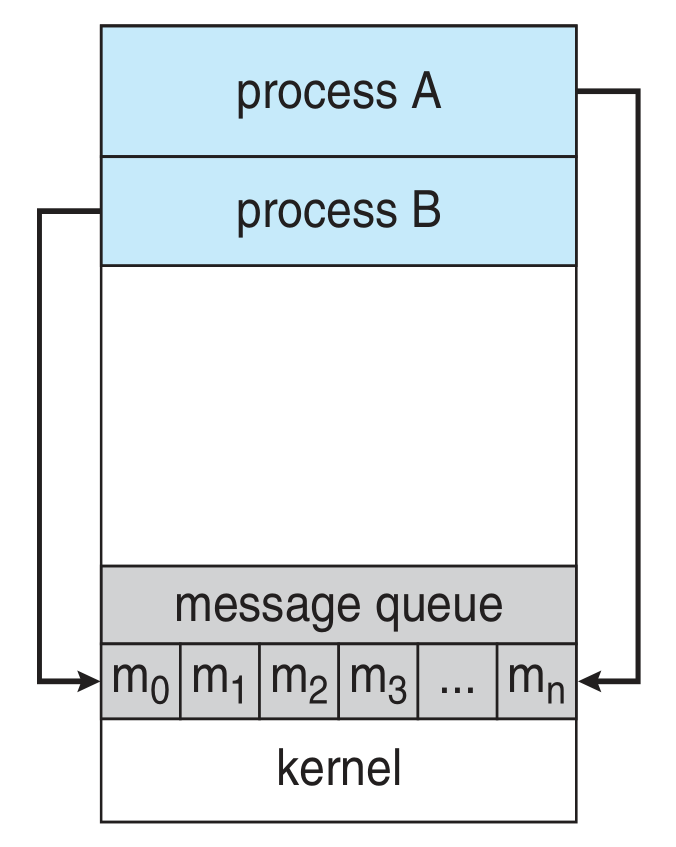
\includegraphics[width=0.2\textwidth]{ipc-message-passing}
		\caption{Diagram of message passing}
		\label{fig:ipc-message-passing}
	\end{figure}

\end{easylist}
\clearpage